\documentclass[11pt,spanish]{article}

% Paquetes
\usepackage{amstext}
\usepackage{amssymb}
\usepackage{babel}
    \addto\shorthandsspanish{\spanishdeactivate{~<>}}
    \decimalpoint
\usepackage[style=iso]{datetime2}
\usepackage{fancyhdr}
\usepackage{float}
\usepackage[T1]{fontenc}
\usepackage[a4paper]{geometry}
    \geometry{verbose,tmargin=3cm,bmargin=2cm,lmargin=2.5cm,rmargin=2.5cm}
\usepackage{graphicx}
\usepackage[utf8]{inputenc}
\usepackage{lastpage}
\usepackage{mathptmx}
\usepackage{units}

% tipo de fuente 
\usepackage{lmodern}

\pagestyle{fancy}
\lfoot{\small DF, FCEyN, UBA}
\cfoot{\tiny Actualizado el {\today} a las {\DTMcurrenttime}}
\rfoot{\small Pág. {\thepage} de \pageref{LastPage}}

\begin{document}

% Título
    \begin{center}
    \textsc{\large Física 2 (Física) -- Cátedra Diego Arbó}
    \par\end{center}{\large \par}
    
    \begin{center}
    \textsc{\large Primer Cuatrimestre de 2025}
    \par\end{center}{\large \par}
    
    \begin{center}
    \textsc{\large Guía 2: Sistemas Acoplados Discretos}
    \par\end{center}{\large \par}

% Comienzo 
\begin{enumerate}

    \section*{Sistemas con más de un grado de libertad}

% Ejercicio 1

    \item Considere el sistema de la figura en ausencia de gravedad

    \begin{figure}[H]
        \centering{}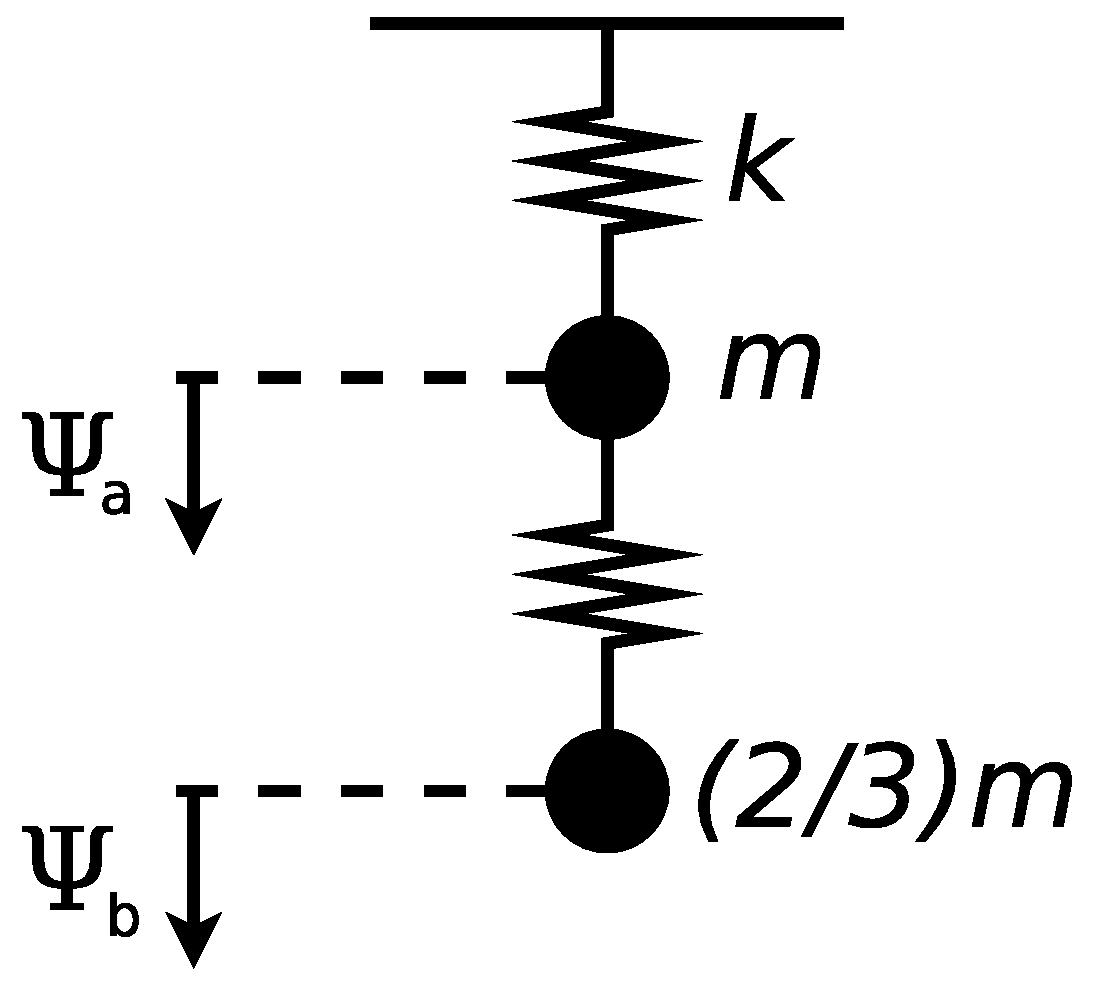
\includegraphics[clip,scale=0.25]{figs/ej1-6}
    \end{figure}

    \begin{enumerate}
        \item Obtenga sus frecuencias naturales de oscilación y los modos
        normales correspondientes. Escriba las ecuaciones de movimiento de cada
        masa.

        \item Sabiendo que a $t=0$ el sistema satisface las siguientes
        condiciones: $\Psi_\text{a}(0)=1,\,\Psi_\text{b}(0)=0$ y que se
        encuentra en reposo, encuentre el movimiento de cada partícula.

        \item Analice cómo se modifica el resultado por la presencia de la
        gravedad.
    \end{enumerate}

% Ejercicio 2

    \item Considere el sistema de dos péndulos de igual longitud $l$ pero de
    masas diferentes $m_\text{a}$ y $m_\text{b}$, acoplados mediante un resorte
    de constante $k$. 

    \begin{figure}[H]
        \centering{}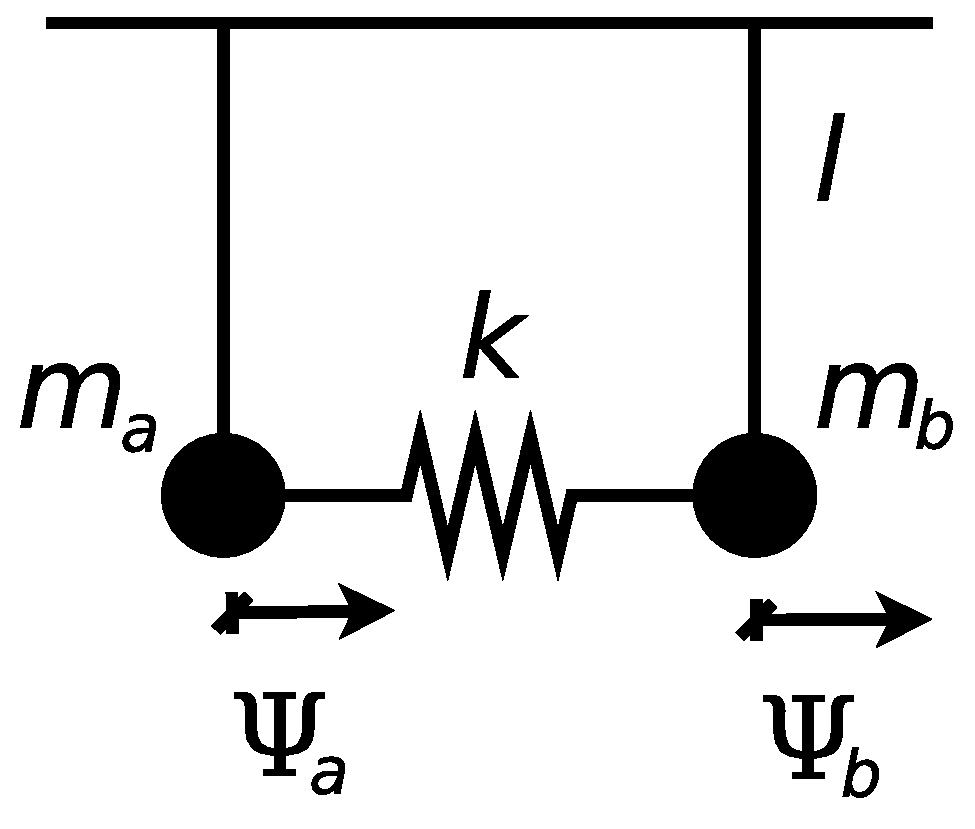
\includegraphics[clip,scale=0.3]{figs/ej1-7}
    \end{figure}

    \begin{enumerate}
        \item Escriba las ecuaciones de movimiento de cada masa.

        \item Obtenga las frecuencias naturales del sistema y sus modos normales
        de oscilación. Interprete el significado físico de estos modos normales.

    \end{enumerate}

% Ejercicio 3

    \item Considere el sistema de la figura. Las masas están apoyadas en una 
    mesa sin rozamiento, sujetas a las paredes por resortes de constante $k$ y
    unidas por otro resorte de constante $k'$. Obtenga las frecuencias y los
    modos transversales del sistema. 

    \begin{figure}[H]
        \centering{}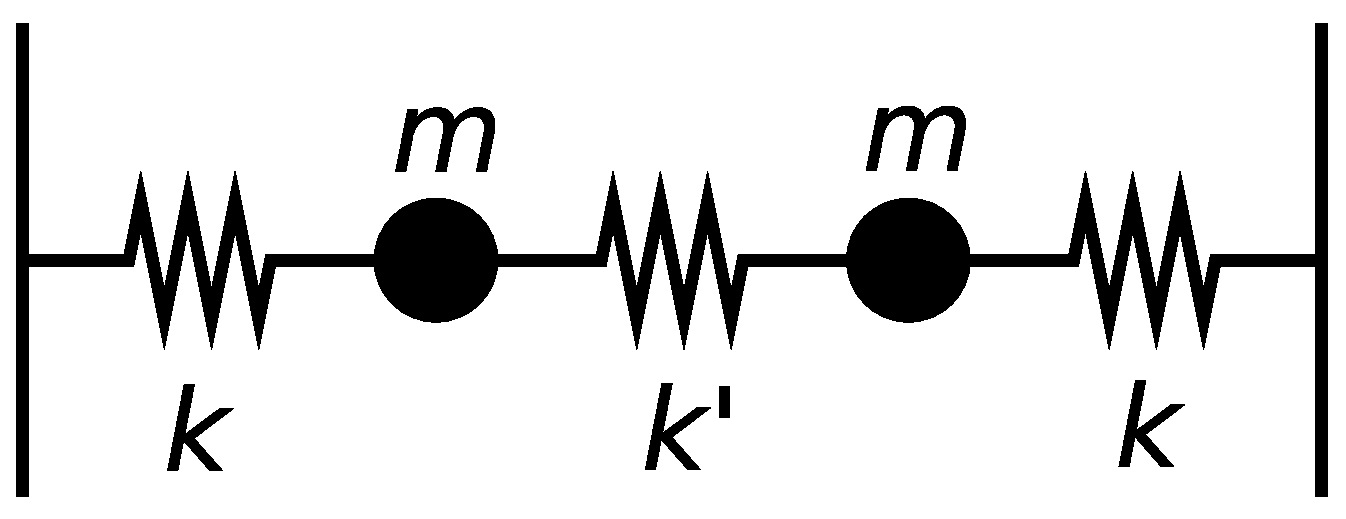
\includegraphics[clip,scale=0.25]{figs/ej1-8}
    \end{figure}

% Ejercicio 4

    \item Considere el sistema simplificado de la figura que se basa en una
    molécula triatómica simétrica. En el equilibrio dos átomos de masa $m$
    están situados a ambos lados del átomo de masa $M=2m$ y vinculados por
    resortes de constante $k$ y longitud natural $l_{0}$. Como sólo estamos
    interesados en analizar los modos longitudinales, supondremos que las masas
    se encuentran dentro de una canaleta que impide todo tipo de movimiento en
    la dirección transversal. 

    \begin{figure}[H]
        \centering{}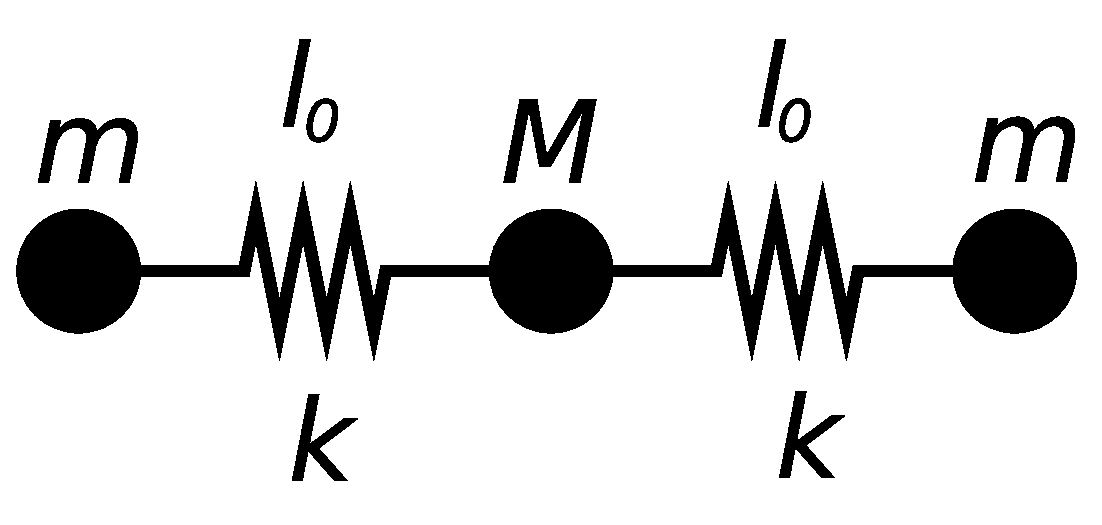
\includegraphics[clip,scale=0.25]{figs/ej1-9}
    \end{figure}

    \begin{enumerate}
        \item Encuentre las ecuaciones de movimiento de cada masa. 
        \item Halle las frecuencias de los modos normales. 
        \item Dibuje las configuraciones de cada modo. 
        \item Establezca cuáles deben ser las condiciones iniciales para excitar
        sólo el modo más alto (mayor frecuencia).
    \end{enumerate}

% Ejercicio 5

    \item Considere el sistema de la figura, en la que los resortes verticales
    tienen longitud natural $l_{0,1}$ y constante $k_{1}$, y los horizontales
    tienen longitud natural $l_{0,2}=0$ (\textit{slinkies}) y constante $k_{2}$.

    \begin{figure}[H]
        \centering{}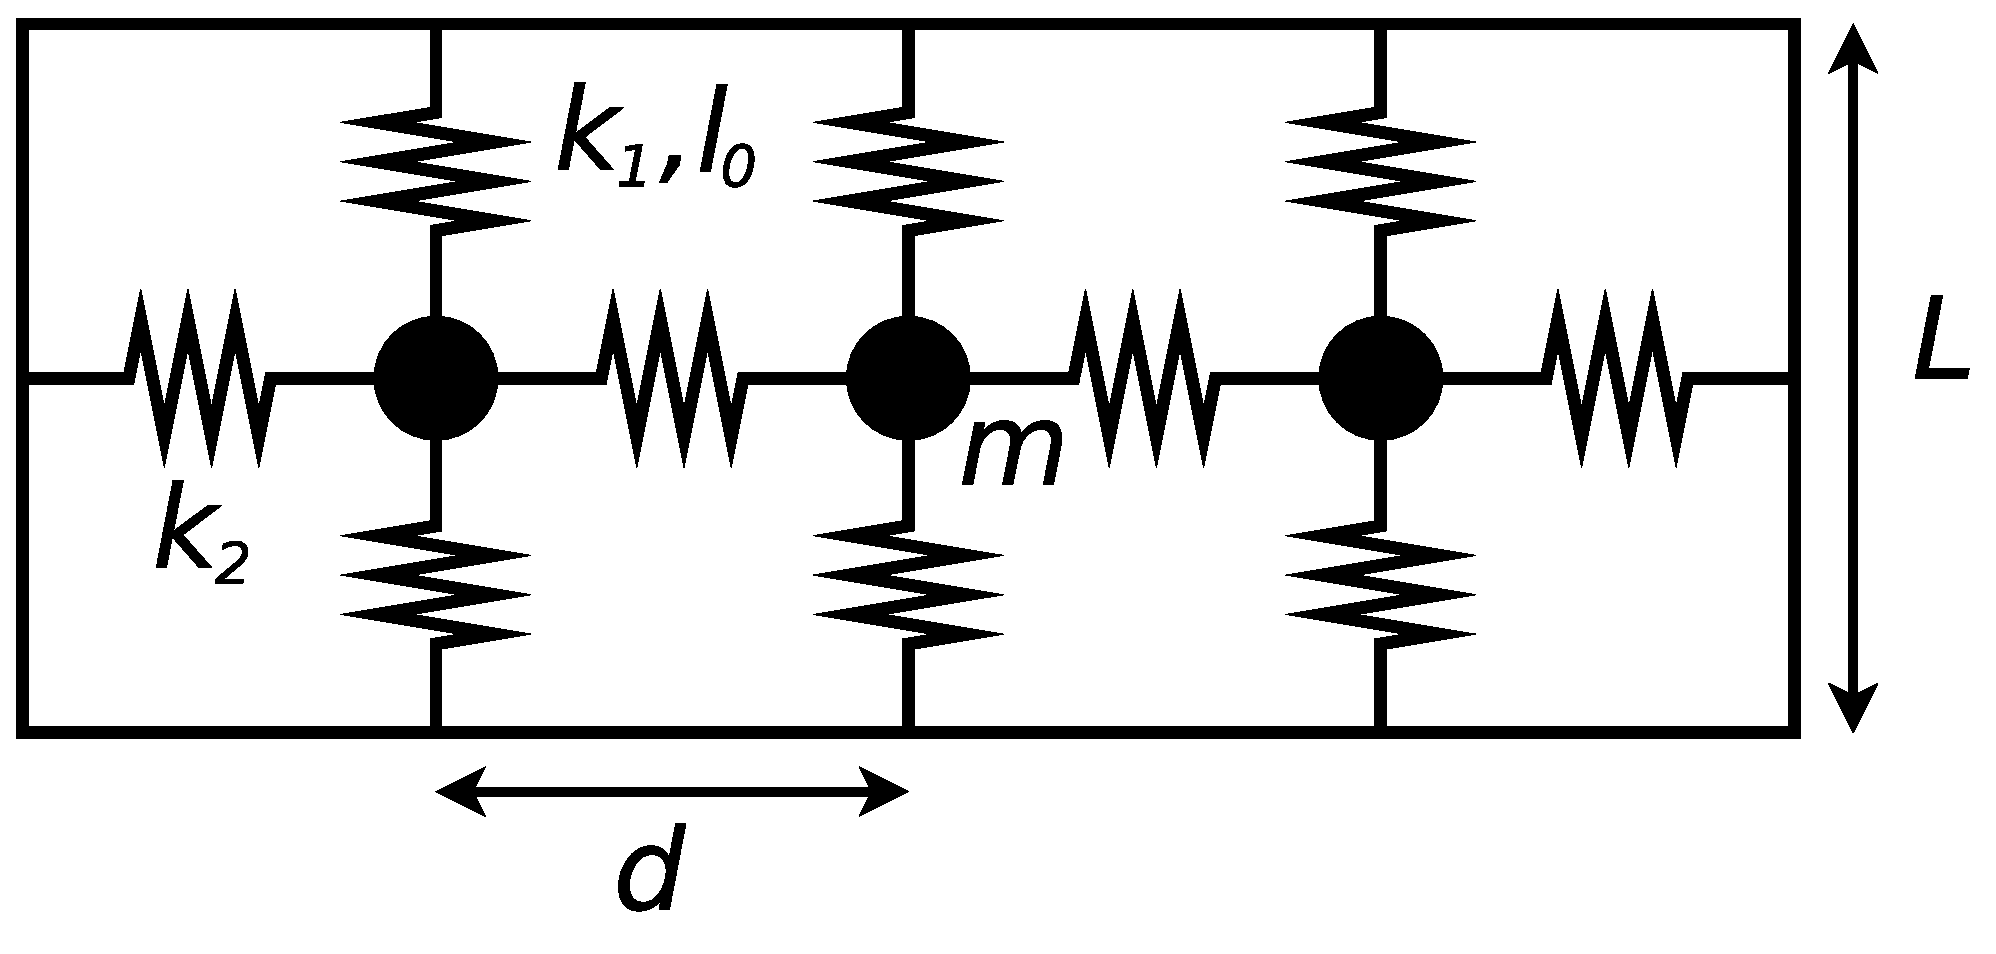
\includegraphics[clip,scale=0.25]{figs/ej1-10}
    \end{figure}

    \begin{enumerate}
        \item Calcule las frecuencias propias y los modos normales.

        \item Considere que las condiciones iniciales son tales que el sistema
        oscila horizontalmente, estando su movimiento descripto por una
        superposición de los dos primeros modos. Halle la energía cinética de
        cada masa y la energía potencial del sistema, el promedio temporal de
        las mismas y la frecuencia de pulsación $\omega_\text{p}$.
    \end{enumerate}

    \begin{description}
        \item [{Datos:}] $l_{0,1}$, $k_{1}$, $l_{0,2}$, $k_{2}$, $L$, $d$,
    $m$.
    \end{description}


    \section*{Acoplamiento débil, pulsaciones y forzado}

% Ejercicio 6

    \item Considere el problema (visto en la sección anterior) de dos péndulos
    de igual longitud $l$ y de diferentes masas, $m_\text{a}$ y $m_\text{b}$,
    acoplados por un resorte de constante elástica $k$:

    \begin{enumerate}
        
        \item Suponiendo que el acoplamiento es débil (es decir:
        $k \ll \frac{g}{l} \frac{m_\text{a}m_\text{b}}{m_\text{a}+m_\text{b}}$)
        y que las condiciones
        iniciales son $\dot{\Psi}_\text{a}(0)=0$, $\dot{\Psi}_\text{b}(0)=0$, 
        $\Psi_\text{a}(0)=0$, y $\Psi_\text{b}(0)=1$; obtenga el movimiento de
        cada masa y grafíquelo en función del tiempo.

        \item Calcule los valores medios, en un ciclo rápido, de $T_\text{a}$ y
        $T_\text{b}$, donde $T$ indica energía cinética. Grafique
        $\left\langle T_\text{a}\right\rangle$ y
        $\left\langle T_\text{b}\right\rangle$, y analice las diferencias en
        el gráfico como función de las diferencias entre las masas
        ($m_\text{a}=m_\text{b}$ y $m_\text{a}$ muy diferente de $m_\text{b}$).
        Calcule el valor medio de la energía de interacción entre las dos
        partículas.    
    \end{enumerate}    

% Ejercicio 7

    \item Considere el sistema del problema 3 de la sección anterior, formado
    por dos masas apoyadas en una mesa sin rozamiento, sujetas a las paredes por
    resortes de constante $k$ y unidas por otro resorte de constante $k'$. ¿Bajo
    qué condiciones espera observar batidos? ¿Qué son los batidos?

% Ejercicio 8

    \item Considere el sistema de dos péndulos acoplados, tal que uno de ellos
    es impulsado por una fuerza $F=F_{0}\cos(\Omega t)$. Desprecie el
    amortiguamiento. Muestre que:
    \[
    \Psi_\text{a}\approx\frac{F_{0}}{2M}\cos(\Omega t)\left[\frac{1}{\omega_{1}^{2}-\Omega^{2}}+\frac{1}{\omega_{2}^{2}-\Omega^{2}}\right];
    \]
    \[
    \Psi_\text{b}\approx\frac{F_{0}}{2M}\cos(\Omega t)\left[\frac{1}{\omega_{1}^{2}-\Omega^{2}}-\frac{1}{\omega_{2}^{2}-\Omega^{2}}\right];
    \]
    \[
    \frac{\Psi_\text{b}}{\Psi_\text{a}}\approx\frac{\omega_{2}^{2}-\omega_{1}^{2}}{\omega_{2}^{2}+\omega_{1}^{2}-2\Omega^{2}};
    \]
    donde $\omega_{1}$ es la menor de las frecuencias modales, $\omega_{2}$
    es la mayor y $\Omega$ es la frecuencia de excitación.

% Ejercicio 9

    \item Considere nuevamente el problema 3 de la sección anterior, pero en
    este caso considere las oscilaciones longitudinales.
    
    \begin{enumerate}
        \item Halle la solución estacionaria para el caso forzado en el cual se
        aplica una fuerza oscilante $F(t) = F_0 \cos(\omega t)$ sobre la masa de
        la izquierda. ¿Qué resonancias espera ver si realiza un barrido de
        frecuencias?
        
        \item Repita el ítem anterior considerando además una fuerza de
        disipación proporcional a la velocidad.
        
        \item Repita el problema para las oscilaciones transversales del sistema.
    \end{enumerate}

    \section*{Sistemas con muchos grados de libertad}

% Ejercicio 10

    \item Considere el sistema de $N$ masas mostrado en la figura. 

    \begin{figure}[H]
    \begin{centering}
        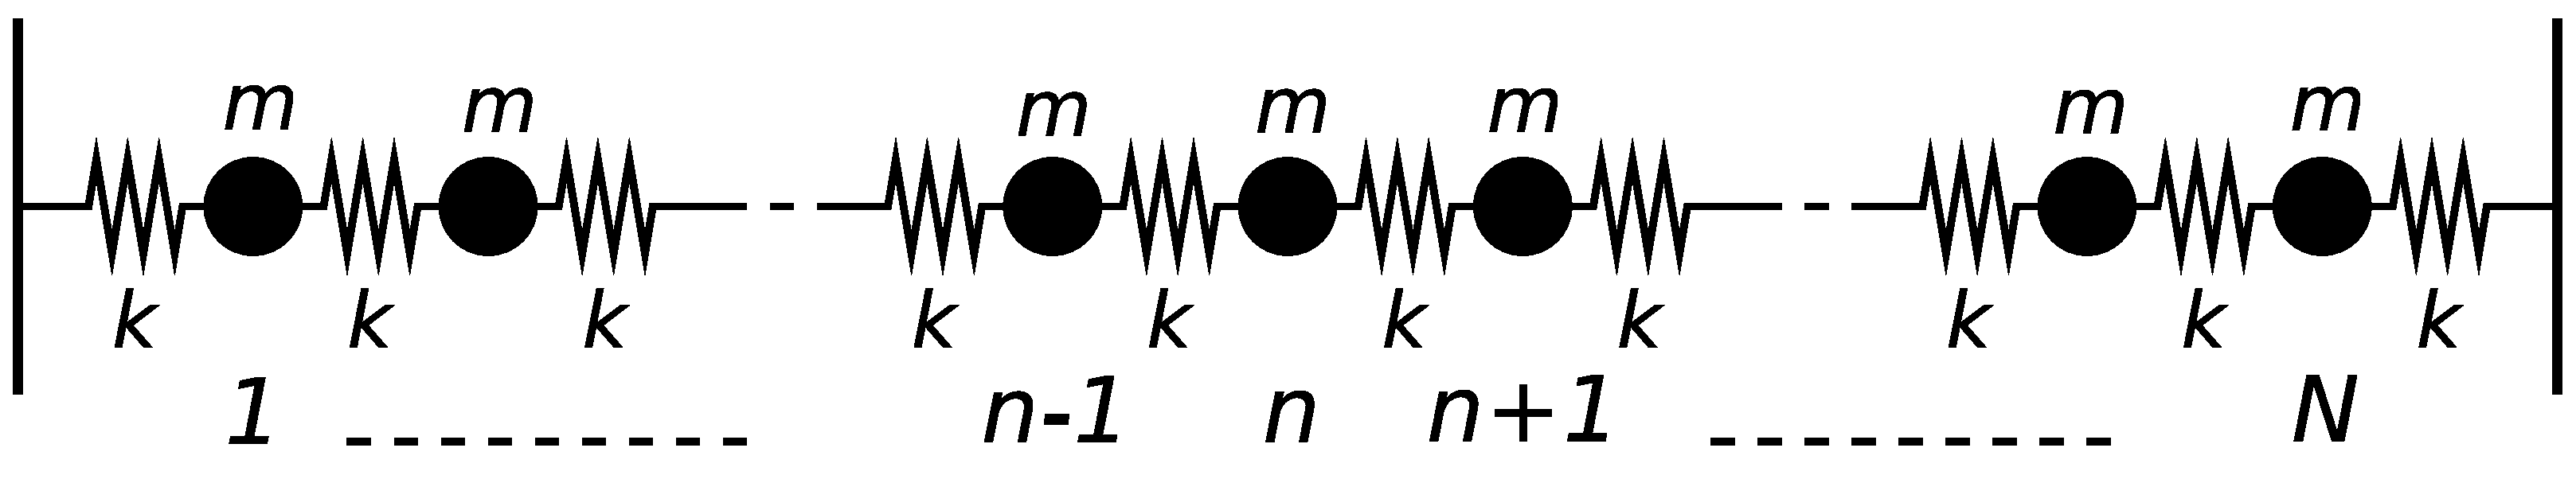
\includegraphics[clip,scale=0.25]{figs/ej1-11}
    \par\end{centering}
    \end{figure}

    \begin{enumerate}
        \item Usando la aproximación de pequeños ángulos, escriba la ecuación de
        movimiento transversal para la partícula enésima.

        \item Proponga una solución de la forma:
        \[
        \Psi_{n}^{(p)}(t)=A^{(p)}\cos\left(nk^{(p)}a+\alpha^{(p)}\right)\cos\left(\omega^{(p)}t+\phi^{(p)}\right)
        \]
        Halle la relación de dispersión y grafíquela. ¿Depende esta relación de
        las condiciones de contorno? ¿Cuánto vale la frecuencia más baja? ¿Qué
        representa dicho modo? 

        \item Obtenga las frecuencias correspondientes a los modos normales
        cuando ambos extremos están libres (atención: ¿cómo sería un ``extremo
        libre'' en esta configuración?) y escriba la solución general para la
        masa enésima. 
        
        \item Ídem anterior, pero considerando que el extremo izquierdo está
        libre y el derecho fijo a la pared.

        \item Particularice los resultados de los dos ítems anteriores para el
        caso en que $N=3$.
    \end{enumerate}

% Ejercicio 11

    \item Considere el sistema de péndulos acoplados de la figura. 
    
    \begin{figure}[H]
        \centering{}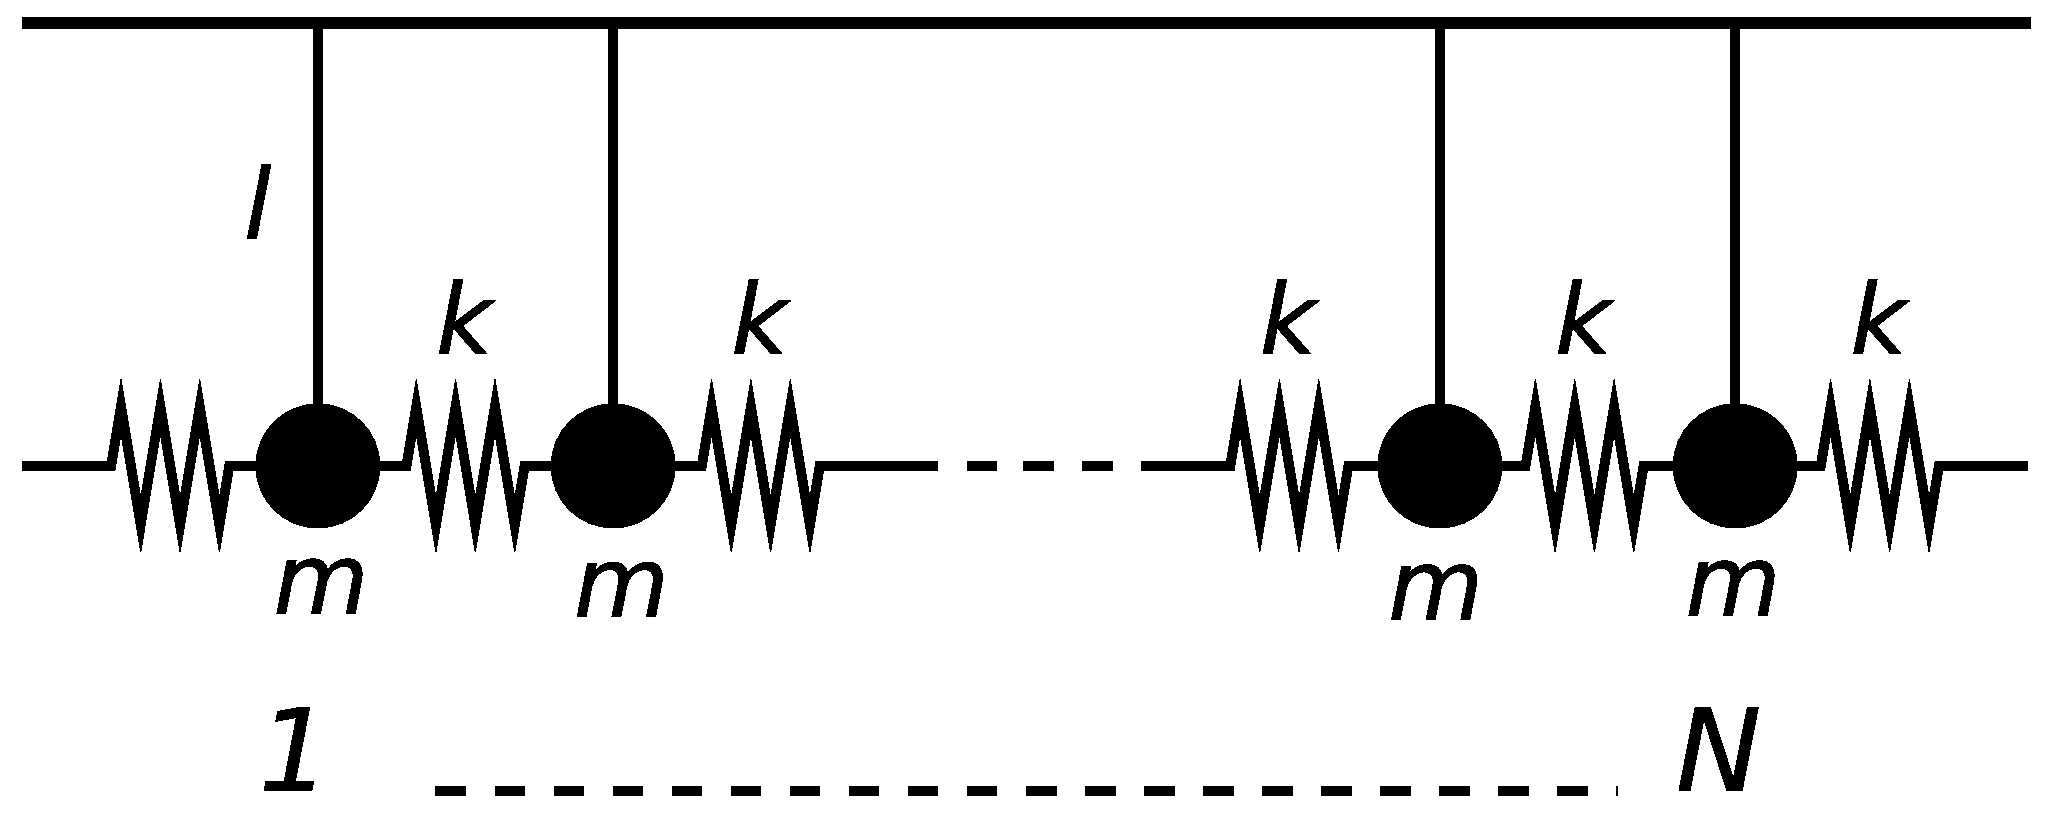
\includegraphics[clip,scale=0.25]{figs/ej1-12}
    \end{figure}


    \begin{enumerate}
        \item Escriba la ecuación de movimiento. Proponga una solución semejante
        a la del problema anterior y halle la relación de dispersión. Compárela
        con la obtenida en el problema anterior. ¿Cuánto vale la frecuencia
        más baja? ¿Qué representa dicho modo?

        \item Obtenga las frecuencias correspondientes a los modos normales
        cuando los resortes de los extremos están fijos y dé las condiciones
        iniciales para excitar el primer armónico.

        \item Idem anterior, pero para el caso en que uno de los resortes de los
        extremos está libre.
    \end{enumerate}

% Ejercicio 12

    \item Considere el sistema de tres péndulos acoplados que se muestra en la
    figura.

    \begin{figure}[H]
        \centering{}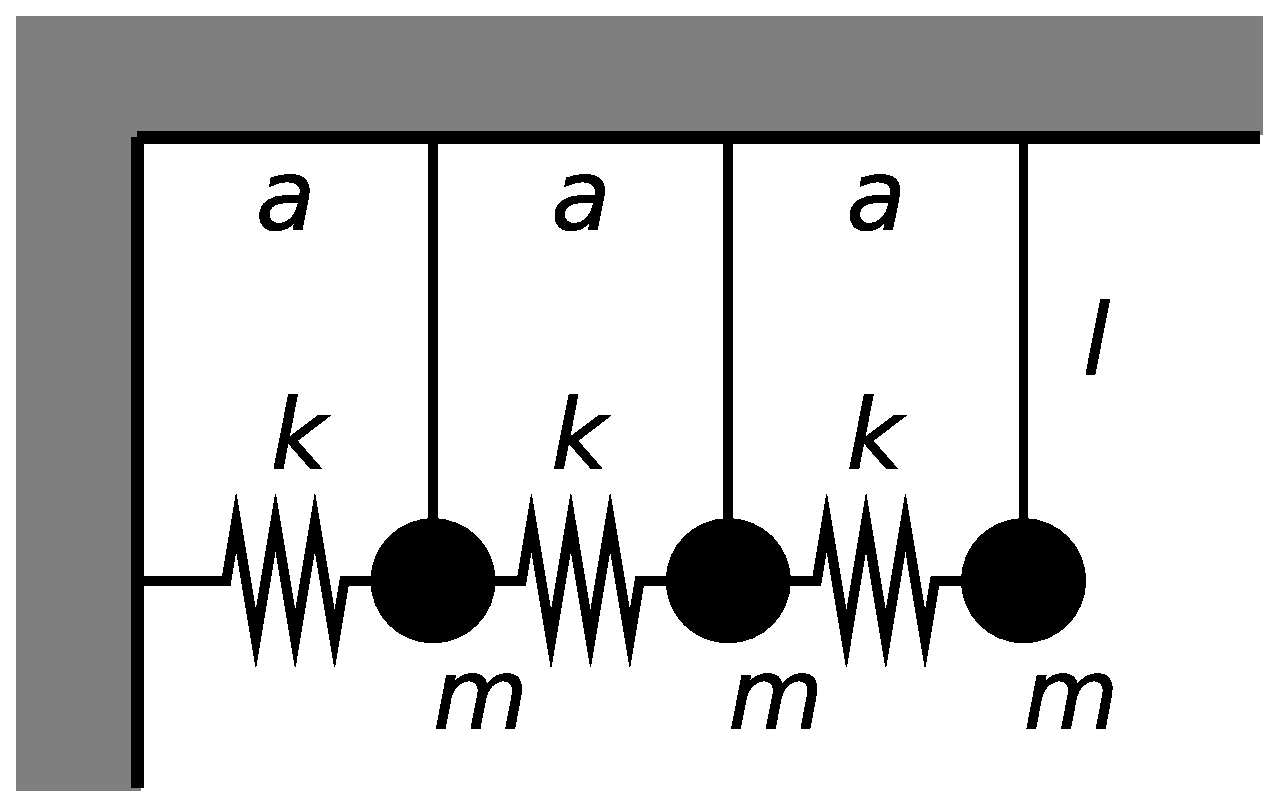
\includegraphics[clip,scale=0.25]{figs/ej1-14}
    \end{figure}

    \begin{enumerate}
        \item Escriba la ecuación de movimiento para cada masa y encuentre las
        frecuencias propias y los modos normales del sistema.

        \item Suponga que en el extremo libre se aplica una fuerza
        $F=F_{0}\cos(\omega t)$. Escriba la ecuación de movimiento para cada
        masa y encuentre la solución estacionaria para cada modo. ¿Cuáles son
        las frecuencias de resonancia?
    \end{enumerate}

    \textbf{Sugerencia:} Use los resultados obtenidos para un sistema de $N$
    péndulos acoplados y particularice la solución para $N=3$. ¿Cómo son las
    condiciones de contorno de este sistema?

\end{enumerate}

\end{document}
